\chapter{Implementation and Core Components of PowerChain} \label{platform}
\label{chapter5}
In this chapter we will present the actual PowerChain implementation. We will describe the technical part including what technologies we used and how we used them.
The actual PowerChain implementation along with all the scripts created, can be found at the following GitHub repository:
\begin{center}
    \url{https://github.com/MnAppsNet/PowerChain}.
    \label{code}
\end{center}

\section{Tools Used}
For the implementation of the actual PowerChain network, we used the ethereum client Geth, which is build in the programming language Go.\cite{geth}
Using Bash scripting language, we build some scripts that are leveraging geth to build a PoA network. These scripts can be used to start a new PowerChain network with any number of validators, depending on the network needs.
For security reasons, and only for the validator nodes, we used clef \cite{clef} which is a tool for signing transactions and data in a secure local environment. Clef can be configured with different rules
to authorize transactions and accesses through RPC on the validator nodes to enhance security. For the purpose of this project, the rules are set to allow all connections to the validator nodes through RPC, for testing purposes.
To interact with the PowerChain network, we build some Python scripts using the Web3.py library \cite{Web3py}. These scripts supports us to deploy smart contracts to the network and to call methods of smart contract
instances. We also build a PowerChain web application using React.Js \cite{Reactjs} and the Web3.js \cite{Web3js} library to interact with the blockchain network.\\
The following scripts have been developed to support with the implementation and management of PowerChain network:\\
\begin{table}[h!]
\centering
\begin{tabular}{c|c|p{8cm}}
    \textbf{Script} & \textbf{Type} & \textbf{Desription} \\
    \hline
    pc\_CreateNetwork & Bash & Initiates a guided procedure to setup and initiate a private PoA network with selected number of validators. For each validator a start script is created to start the node. \\
    \hline
    pc\_CreateBootnode & Bash & Initiates a guided procedure to create a bootnode. It creates a start script that can be used to start the node. \\
    \hline
    pc\_CreateAcount & Bash & Initiates a guided procedure to create a user node. It creates a start script that can start the node. \\
    \hline
    pc\_DeployContract & Python & It gets as parameters the path of a solidity smart contract code and the RPC of a node in the network, compiles the contract, deploys it to the network and produces a contract json file that contains the contract address and interface. \\
    \hline
    pc\_CallPowerChainMethod & Python & It gets as parameters the RPC of a node in the network, the path to the PowerChain contract json (json returned from pc\_DeployContract), a method name from PowerChain, the parameters of the relevant method, calls the PowerChain contract and returns the results. It can also be imported on a python script. \\ 
\end{tabular}
\caption{Scripts to create and manage PowerChain network}
\end{table}\\ 

To simulate the production and consumption of energy in and out of a storage unit, we created a python script (storage\_unit.py). 
This script can be used to simulate a storage unit address with capabilities to produce and consume energy. 
In a real life implementation this role will be handled by an IoT device that monitors the input and output of energy to the batteries of a storage unit.

\pagebreak

\section{PowerChain Commands}
The PoweChain protocol defines a set of commands which are implemented into the blockchain layer using a Smart Contract. It determines when and how are the network tokens minted, burned and transferred. 
It also defines the network participant authorizations. In the network, there are different types of roles with each one authorized to execute different type of commands:
\begin{itemize}
    \item \textbf{The normal user}: This is the default role all network participants have. These users can not execute commands that require voting or commands that burn or mint tokens.
    \item \textbf{The voter}: The voters can execute all the commands a normal user is allowed to execute, with the addition of commands that require voting. Such commands could be for example, the promotion of a user to voter
    or the registration of a new storage unit.
    \item \textbf{The storage unit}: This role is assigned to the smart meters managing the energy of a storage unit and it gives the permission to execute commands that lead to the minting or burning of tokens. They
    can also execute normal user commands.
    \item \textbf{The banker}: This role is assigned to the address of a trusted authority which will be responsible to mint/burn eEuro tokens by moving real world euro in and out of circulation.
\end{itemize}
Below, we analyze the commands each of the mentioned roles can execute.\\
\textbf{Voter Commands}:\\
\begin{tabular}{|p{5.5cm}|p{8cm}|}
    \hline
    Register Storage Unit & Start a vote to register a storage unit, providing the unit and the owner addresses \\ \hline
    Remove Storage Unit & Start a vote to remove storage unit, providing the unit address \\ \hline
    Change Banker & Start a vote to register an address as banker, initially the banker address is the zero address \\ \hline
    Set Parameter & Start a vote to set a network parameter, providing the parameter name and value \\ \hline
\end{tabular}\\

\textbf{Storage Unit Commands}:\\
\begin{tabular}{|p{5.5cm}|p{8cm}|}
    \hline
    Energy Produced & Reports energy production based on the producer address and the wh produced \\ \hline
    Energy Consumed & Reports energy consumption based on the consumer address and the wh consumed \\ \hline
    Report Actual Energy & Reports the actual energy that is available in the storage unit  \\ \hline
\end{tabular}\\

\textbf{Banker Commands}:\\
\begin{tabular}{|p{5.5cm}|p{8cm}|}
    \hline
    Mint eEuro & Mint an amount of eEuro into the provided address. \\ \hline
    Burn eEuro & Burn an amount of locked eEuro from the provided address and give the equivalent real world Euro to the user. Only eEuro locked by the user can be burned. \\ \hline
    Unlock eEuro & Unlock an amount of locked eEuro, locked by the user in order to withdraw the relevant real world Euro amount. \\ \hline
\end{tabular}\\

\textbf{Normal User Commands}:
\begin{longtable}{|p{5.5cm}|p{8cm}|}
    \hline
    Get Total Energy & Returns the total energy of the network \\ \hline
    Get Storage Units & Returns the active storage units of the network \\ \hline
    Get Storage Unit Energy & Returns the total energy of a storage unit \\ \hline
    Get Energy Rates & Returns the ENT minting and burning rates of the network \\ \hline
    Start Consumption Session & Start a consumption session with a storage unit for the defined amount of ENT tokens owned by the user \\ \hline
    Get Consumption Session & Returns the consumption sessions of the caller \\ \hline
    Get Consumption Session Energy & Returns the available energy of a consumption session, providing the address of the session counterpart \\ \hline
    Get Storage Unit Info & Returns the state, the owner and the available wh of a storage unit based on its address \\ \hline
    Clear Old Sessions & Clear old sessions that have been expired \\ \hline
    Get Parameters & Returns the network parameters \\ \hline
    Get total ENT & Returns the total amount of ENT in circulation \\ \hline 
    Get total eEuro & Returns the total amount of eEuro in circulation \\ \hline
    Get ENT balance & Returns the amount of locked and unlocked ENT tokens \\ \hline
    Get eEuro balance & Returns the amount of locked and unlocked eEuro tokens \\ \hline
    Transfer ENT & Transfer an ENT amount to the provided address \\ \hline
    Transfer eEuro & Transfer an eEuro amount to the provided address \\ \hline
    Lock eEuro & Lock an amount of eEuro, making burnable by the banker. The banker can then burn the tokens and give the equivalent amount of real world Euro to the user. \\ \hline
    Add Order & Add an order in the orderbook to buy ENT based on required price per unit \\ \hline
    Remove Order & Removes an order from the orderbook \\ \hline
    Get Orders & Returns a list of available orders in the network \\ \hline
\end{longtable}

\section{Network Parameters}
\label{networkParameters}
PowerChain smart contract, defines some parameters that influence the network behavior. These parameters can be modified by the voters, based on the needs of the network participants. 
The mentioned network parameters are the following:
\begin{itemize}
    \item \textbf{M} : Maximum minting cost. This is the maximum ENT cost per kWh to be applied when energy is produced.
    \item \textbf{B} : Maximum burning cost. This is the maximum ENT cost per kWh to be applied when energy is consumed.
    \item \textbf{C} : Missing energy recover rate. This parameter defines how fast will the ration between total energy and total ENT in circulation will return to 1 in case of misalignment.
    \item \textbf{H} : Consumption session validity period. This is the amount of hours a consumption session will remain valid. After the validity period the consumption session is closed and any remaining assets are returned to the owners.
    \item \textbf{F} : Storage provider fee. This is the percentage of the total ENT minted by an energy producer, to be rewarded to the storage provider.
\end{itemize}
These network parameters should be defined carefully in order to incentivize the network peers to participate in the network and provide a fare token distribution.
In case of a big misalignment between the total ENT in circulation and the total energy in the network, parameters M and B are used to make sure that producers are receiving a minimum fare amount of ENT and consumers are not spending too much ENT for their 
energy needs, until the network reaches again equilibrium. Parameter C controls how fast we reach a ratio of 1 between total ENT and total energy, by burning some extra ENT during consumption or minting a fewer ENT during production. A big C value, means that 
we will reach a balance quicker but each individual network participant will have to cover a bigger part of the energy loss through a higher minting/burning cost, potentially splitting the cost to fewer participants. On the other hand, if parameter C is too small, 
the cost to return network in balance is smaller per kWh produced or consumed but network will reach equilibrium slower. Parameter H was introduced to avoid having consumption session assets locked forever. Consumption session will remain valid within the time frame defined by H. 
Finally, parameter F controls what percentage of ENT, from the ENT minted by a producer, should a storage provider keep, for providing its batteries. These parameters have some default values and can be then adapted based on the network needs. The default parameter values are the following:
\begin{itemize}
    \item \textbf{M} = 0.5 ENT / kWh
    \item \textbf{B} = 0.5 ENT / kWh
    \item \textbf{C} = 5 \% of the loss covered each minting / burning (step), equilibrium is reached in at least 20 steps
    \item \textbf{H} = 2 Hours until consumption session becomes invalid
    \item \textbf{F} = 20 \% of minted ENT tokens are kept by storage provider
\end{itemize}

\section{PowerChain Voters}
The PowerChain contract voters have a crucial role in the maintenance and smooth operation of the energy trading network.
They are responsible to audit and agree on the new voters and storage units to be included in the network. They have also
the responsibility to monitor the network and propose new network parameter values that could benefit the participant.\\
As we already mentioned on the previous sections, PowerChain has a set of voter commands. These are a special
kind of commands as they are not directly executable. Every time a voter executes one of these commands, a voting procedure starts with one
positive vote from the voter that executed it. The actual action of the command is not executed until the vote is passed. Whenever another voter 
executes the same command with the same parameters, it agrees with the vote and another positive vote is counted. If the same command with the same parameters 
is executed again by the same voter, the vote changes to a negative vote. For simplicity reasons and in order to keep the voting process fair, we defined that a vote is passed if it has 
more positive votes than the number of voters in the network divided by 2.
\begin{empheq}[box=\fbox]{align}
    \label{equ:vote_pass}
    \text{Vote Passed when: } V_+ / N > 0.5
\end{empheq}
Where,\\
\begin{tabular}{rl}
    $V_+$ & :  Number of positive votes. \\
    $N$   & :  Total number of voters \\
\end{tabular}\\
The voter that adds the last positive vote which  marks the voting as passed, is also executing the action of the command and the voting process is concluded.

\section{PowerChain Web Application}
The PowerChain web application allows the network users to interact easily with the PowerChain contract, though a user interface.
The web application is a control panel that consists of four basic sections and two special ones. To connect the web application with the blockchain network, we make use of MetaMask which works as a blockchain wallet \cite{metamask}.
More details are presented below for each section.
\begin{figure}[h!]
    \centering
    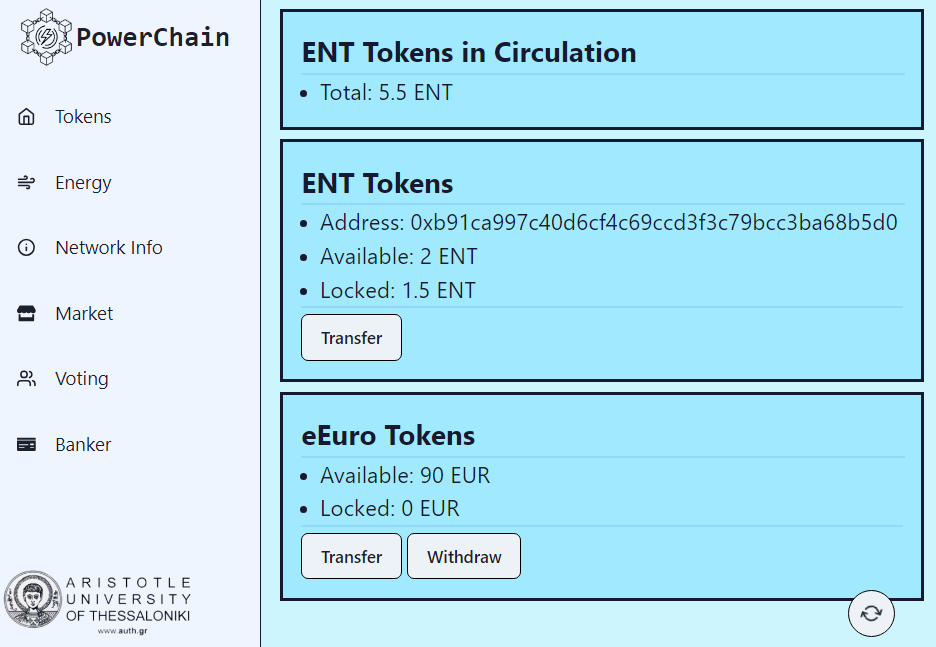
\includegraphics[width=\linewidth,frame,scale=1]{Figures/webapp.png}
    \caption{PowerChain Web Application}
\end{figure}
\begin{itemize}
    \item \textbf{Tokens}: This section provides an overview of the user's tokens and it gives also the possibility to transfer the tokens.
    \item \textbf{Energy}: In this section more information about the network's energy are provided. We can see the available storage units and the amount of energy they contain in kWh.
    There is also the option to start a new consumption session with a storage unit and start consuming energy.
    \item \textbf{Network Info}: In this section more network information are provided to the user like the banker address, the total eEuro in circulation and even the values of the network parameters.
    \item \textbf{Voting}: This is a special section that is only available to the users with the voter role. It provides an overview of the user's votes and gives the possibility to start a new vote.
    \item \textbf{Banker}: This is also a special section that is available only to the banker address. It gives the option to mint, burn and unlock eEuro tokens.
\end{itemize}

\section{Summarization}
In this chapter we went through the core components of our proposed energy trading solution, PowerChain. We discussed about the tools we used to make the implementation happen and the scripts 
we created to help us maintain and manage the PowerChain network. We analyzed the PowerChain smart contract and presented the available commands it offers. We also explored some network parameters that
can influence the network behavior and can be adapted based on the participant needs. Finally, we talked about the voter role defined by the PowerChain protocol and the web application that can be used
to access the PowerChain commands.
